\documentclass[a4paper,12pt]{article}
\usepackage{url}
\usepackage{epsfig}
\usepackage{graphics}
\usepackage{fancyhdr}
% -- algoooo
\usepackage[]{algorithm}
\usepackage{float}
\usepackage{algpseudocode}
\usepackage{setspace}

\usepackage{hyperref}
\graphicspath{{pictures/}}


\title{Training a Convolutional Neural Network for Phonemes Classification}
\author{\hspace*{-0.5cm}
\begin{tabular}{cccc}
Mohamed Abdulaziz Ali Haseeb & Omar El-shenawy \\
moaah@kth.se & omares@kth.se %\\
%\includegraphics[width=0.13\linewidth]{Alan_Turing_photo} & 
%\includegraphics[width=0.13\linewidth]{Alan_Turing_photo}
\end{tabular}} 
% Normally there will not be any pictures but we want
% these so that we can connect faces to names in the course
% We also want birthdates so that we can tell people with the same
% name apart
\date{}

\pagestyle{fancy}
\setlength{\headheight}{15pt}
\fancyhf{}
\lhead{DT2118 2015} % DO NOT REMOVE!!!!
\rhead{M. Haseeb, Omar El-shenawy} %% UPDATE WITH YOUR NAMES

\begin{document}

\maketitle
\thispagestyle{fancy}
\begin{abstract}
Convolutional Neural Networks has interesting properties that make them more suitable to cope with spectral variations and model spectral correlations. In this report we present our work on training a deep convolutional neural network CNN for phoneme classification acoustic task. CNNs with different configurations are trained and compared.
\end{abstract}
\clearpage
\section{Introduction}

Neural networks have always been an attractive area of research since 1960. The attempt at simulating the human brain has always been intriguing. Since the first perceptron model, Neural Networks have evolved in many ways, in which layers of perceptrons grew wider and deeper. However, until recently, it was only possible to train shallow networks, because of the vanishing gradient problem. The vanishing gradient is a phenomena where the error information starts to decay when propagated through many layers, and therefore the learning process is no longer doable. A remedy was made by Hinton\cite{hinton2006reducing}, in which the network is trained a layer at a time, instead of trying to train all layers at once.\\\\
Deep Learning is the new trend in Machine Learning field. Recently, there has been many applications that uses Deep Learning. Training these deep networks is very expensive computationally, they require heavy computations on the GPU, and so far, several frameworks that facilitate training Deep Neural Networks (DNN) and Convolutional Neural Networks (CNN) ---a deep network that uses Convolutional filters--- have been developed by many research labs around the world. CNNs are usually very popular with the computer vision applications.\\\\
Recently, DNNs and CNNs have been applied to the field of speech recognition with very promising results. CNNs have the ability to reduce spectral variations and model spectral correlations which exist in signals, therefore CNNs are a more effective model for speech compared to DNNs \cite{sainath2013deep}. In this work, we experiment with CNNs and apply them to a small scope of acoustic modelling which is phoneme classification, using the TIMIT dataset. We use the CNN training library, Caffe to train our network. We train on spectrograms i.e. images of Fast Fourier Transform applied on the phonemes acoustic data. We base our work on the architecture described in \cite{sainath2013deep}.

\section{Related Work}
There has been many approaches for speech recognition with Neural Networks. The classical approach was always to combine Hidden Markov Models (HMMs) with NNs, such as \cite{robinson1994application}. This approach has been very successful and popular. Recently, there has been attempts to remove the need for HMMs. \cite{graves2013speech} used Recurrent Neural Networks (RNNs) with good results for speech recognition and has yielded promising result. \cite{graves2014towards} have done similar work with RNNs.\\\\
\cite{sainath2013deep} uses HMMs in their model, however, we only build a CNN based on their architecture, and since we do not do speech recognition, there is no need for an HMM.\\\\
There has been attempts to use both DNNs and CNNs in speech recognition, however, DNNs have difficulty modeling transitional variance within speech signals, which exists due to difference in speaking styles \cite{lecun1995convolutional}. Various speaker adaptation techniques are required to reduce this variation. Therefore, we have preferred to use CNNs for this task, since TIMIT consists of a wide range of speakers.

\section{Method}
In the section the approach followed to build the CCN will be described.
\subsection{Overall setup}
A deep CNN will be trained to give a probability distribution over the phonemes labels given the acoustic input. The acoustic input will be converted into a sequence of fixed size frames windows, that is converted into spectrograms. The deep CNN will then generate probability distributions over the possible phone labels for each spectrogram. The sequence of the probability distributions will then be used to compute the emission probabilities of the HMM states on a Viterbi decoder that can generate the expected phones sequence.\\\\
In this work, the CCN network ability to predict the correct phone label given an input spectrogram was tested, and no Viterbi decoder was used.
\subsection{Feature representation}
As in \cite{graves2014towards} we have chosen to use the spectrograms as inputs to the CCN. The acoustic input are split into smaller frames chunks which are then converted into fixed size spectrogram images. Section \ref{sec:spect} detail the spectrograms generation process for this phone recognition task.

\subsection{Network Architecture}
As suggested in \cite{sainath2013deep}, a CNN network with both convolutional layers and fully connected layers cwill be used. The convolutional layers will be used at the lower layers of the network, while the fully. connected layers will be used at the top layers of the network. The convolutional layers will be followed with pooling layer. Having the convolutional layers at the bottom of the network helps with the spectral variation, and the fully connected layer are used to discriminate between the different phonemes using the convoluted-pooled input from the convolution and pooling layers.
\subsection{Evaluation}
A number of CNN with different number of layers will be trained. The performance of these networks will be compared using the classification error rate. Due to the limitation of the computing resources, a relatively small networks will be trained, also the network will be trained to classify over a subset of the phonemes.

\section{Dataset}\label{sec:spect}
The Timit corpus \cite{timit} was used for verifying the proposed solution. It contains recordings of 630 speakers from 8 different regions in the united states. Each speaker read 10 sentences, recorded at 16 KHz frequency. Beside the audio recordings, the corpus contains time-aligned orthographic, word and phonetic transcription.\\\\
To create the spectrogram images that are used as input to our phone recognition network, the phonetic time alignment information are used to extract the frames associated with each phoneme. The frames of each phoneme are then split into 16ms Hanning windows with 15.5 ms overlap. A Fast Fourier Transform is then applied on the frames to generate a spectrogram, which are then padded to create a 128 by 128 pixels images. Figures \ref{fig:spec1} and \ref{fig:spec2} shows example spectrograms.
\begin{figure}[H]
\centering
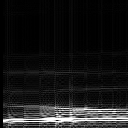
\includegraphics[width=0.6\linewidth]{figs/ao.png}
\caption{Spectrogram of phoneme \textbf{ao}}
\label{fig:spec1}
\end{figure}
\begin{figure}[H]
\centering
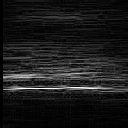
\includegraphics[width=0.6\linewidth]{figs/sh.png}
\caption{Spectrogram of phoneme \textbf{sh}}
\label{fig:spec2}
\end{figure}

\section{Experiments and Results}
\subsection{Implementation}
\label{sec:impl}
The Timit corpus contains 6300 \textbf{wav} files corresponding to the 6300 sentences uttered by the 630 different speakers. The \textbf{Sndfile} from \textbf{scikits.audiolab} library is used to read the \textbf{wav} files. Using the phones time alignment information, the frames of each phoneme are extracted and saved as \textbf{wav} files, resulting a \textbf{wav} for each phoneme. The \textbf{wav} files are then converted into spectrogram images using a script provided by \cite{pannous}.\\\\
The CCN network was built and trained using the NVIDIA DIGITS deep learning system \cite{digits}. DIGITS provides web based user interfaces that wraps the Caffe deep learning framework \cite{caffe}. The training was done on rented Amazon instance that has a GPU with around 1500 cores. The trained model is then used tested using Caffe pycaffe module, since DIGITS provides poor testing facilities.
\subsection{Experiments}
\label{sec:experiments}
The original 61 phonemes in the TIMIT corpus was mapped into 39 phonemes as suggested in {mapping}. This mapping is shown in table \ref{table:mapping}. The 39 phonemes are then used to both train and evaluate the model. 
\begin{center}
\begin{table}[H]
    \begin{tabular}{ | l | l |}
    \hline
    aa, ao & aa \\ \hline
    ah, ax, ax-h  & ah \\ \hline
    er, axr & er \\ \hline
    hh, hv & hh \\ \hline   
    ih, ix & ih \\ \hline
	l, el & l \\ \hline
	m, em & m \\ \hline
	n, en, nx & n \\ \hline
	ng, eng & ng \\ \hline
	sh, zh & sh \\ \hline
	uw, ux & uw \\ \hline
	pcl, tcl, kcl, bcl, dcl, gcl, h\#, pau, epi & sil \\ \hline
	q & - \\ \hline
    \hline
    \end{tabular}
    \caption{Mapping the 61 original TIMIT phonemes(left) into 39 phonemes(right) as suggested in \cite{mapping}}
    \label{table:mapping}
\end{table}
\end{center}


we tried different networks 
different data sets (train/validation split)
results, including training time
in a table
\section{Discussion and Conclusions}
The method showed good potential in separating two phonemes, this was very beneficial as a proof of concept to show that the model works. However, as seen from results in Table~\ref{table:unseen}, our method was unable to generalize with good performance. However on the validation set, it was able to perform very well. The reasons behind this difference in performance is still unknown to us, however we propose some possible explanations and future work.

\begin{itemize}
\item The size and complexity of the network. Through all experiments, we were never able to get our model to overfit the data, this suggests that our model might not be complex enough. Another explanation is that the model needs much more epochs to learn.

\item It might be the size of the spectrograms used. The size we used is small and does not capture variations that differentiate the different phone classes, for instance, Google successfully used words spectrograms.

\item The representation of the data, while it was easily separated in the two phoneme case, the representation might not be separable for the 39 phoneme case. Therefore we might want to experiment with raw sound waves.

\item The amount of data used. Unfortunately, due to the expensiveness of the training, we were only able to train only on 39 phonemes for all regions. Most of the literature trains on all 61 phonemes, and tests on a smaller subset (39 phonemes).

\end{itemize}

\bibliographystyle{acm}
\bibliography{library}

\end{document}